% !TEX encoding = UTF-8
% !TEX TS-program = pdflatex
% !TEX root = tesi.tex
% !TeX spellcheck = it_IT

%**************************************************************
\chapter{La teoria}
\label{cap:teoria}
Per comprendere al meglio le tecnologie e i concetti che avrei dovuto implementare in questo stage ho deciso di avere un approccio il più sistematico possibile alla materia. Essendo la teoria implicata molto ampia e con un approccio matematico non banale, ho deciso inizialmente di leggermi molti articoli, per lo più tratti da \textit{medium.com}\cite{site:medium}, ottimo sito di divulgazione generale. Dopodiché ho frequentato alcuni corsi su Coursera\cite{site:coursera}, famoso sito di corsi online.
\medskip
\\In particolare, ho seguito buona parte del corso sul \textit{machine learning}\cite{course:machine-learning} tenuto da Andrew Ng\cite{person:andrew-ng} per avere un'infarinatura generale di cosa vuol dire questo approccio matematico. In seguito per avere un'idea più completa riguardo le \textit{deep networks} mi sono affidato a dei corsi, sempre su Coursera\cite{site:coursera} e tenuti dallo stesso docente, che fanno parte di una specializzazione\cite{course:deep-learning-specialization}. In particolare, ho completato - con certificato - i seguenti corsi:
\begin{itemize}
	\item Neural Networks and Deep Learning\cite{course:neural-networks-deep-learning};
	\item Improving Deep Neural Networks: Hyperparameter tuning, Regularization and Optimization\cite{course:improving-nn};
	\item Structuring Machine Learning Projects\cite{course:structuring-ml-proj};
\end{itemize}
Non sono invece riuscito a concludere gli esercizi finali del quarto capitolo: Convolutional Neural Networks\cite{course:cnn}.
\medskip
\\Tutta questa preparazione mi è stata di fondamentale aiuto per comprendere le tecnologie che sarei andato ad utilizzare di lì a breve, nonché mi ha dato la possibilità di ampliare enormemente la mia conoscenza al riguardo. Nei capitoli seguenti descriverò in maniera più intuitiva che matematica le tecnologie che ho esplorato.

%**************************************************************

%\intro{Brevissima introduzione al capitolo}\\

%**************************************************************
\section{Cos'è l'apprendimento automatico}
L'apprendimento automatico - in inglese \textit{machine learning} - si basa sull'idea che un algoritmo sia capace di dire qualcosa di interessante riguardo un insieme di dati senza la necessità, da parte di un utente, di dover scrivere alcuna riga di codice specifico sul problema.\cite{site:machine_learning_is_fun} L'algoritmo infatti, sulla base di questi dati, è capace di sviluppare una propria logica. Prendiamo ad esempio due task:
\begin{itemize}
	\setlength\itemsep{0em}
	\item riconoscere dei numeri scritti a mano;
	\item riconoscere una mail di spam da una legale.
\end{itemize}
Possiamo sfruttare lo stesso algoritmo di apprendimento automatico per generare due logiche differenti solamente a partire da due \gls{set} di dati diversi.


\subsection{Apprendimento supervisionato e non supervisionato}
Esistono due principali categorie di apprendimento automatico: supervisionato e non supervisionato.\cite{site:supervised_vs_unsupervised_learning}

\subsubsection*{Apprendimento supervisionato}
Il \textit{supervised learning} è principalmente usato per la classificazione, dove vogliamo ottenere delle etichette a partire da dati in ingresso, oppure per la regressione, dove l'input è mappato in un output continuo. In entrambi gli aspetti, l'obiettivo è quello di dedurre una particolare relazione o struttura nei dati di input che ci permetta di produrre un output corretto.

\subsubsection*{Apprendimento non supervisionato}
Con l'\textit{unsupervised learning} si vuole trarre una struttura a partire da dati in ingresso senza fornire esplicitamente un'etichetta. Si usa principalmente per il raggruppamento e le stime di densità di un insieme di dati in input.



\section{Le reti neurali}
Le reti neurali sono una classe di modelli di apprendimento automatico che hanno rivoluzionato il mondo del \textit{machine learning}.
Lo sviluppo delle \textit{neural networks} è stata la chiave per insegnare ad una macchina a \textit{capire} come un umano. 

\subsection*{Cos'è una rete neurale}
La rete neurale si può pensare come una funzione composta. Essa accetta alcuni tipi di input e genera degli output. I componenti della rete neurale sono i \textbf{neuroni} (anche detti \textit{Perceptrons} oppure unità), che a loro volta sono una funzione che utilizza \textbf{pesi} (o anche detti connessioni) e \textbf{\textit{biases}}. Viene poi interpellata una \gls{funzione di attivazione} non lineare per restringere l'output ad un certo intervallo. Se ne immaginassimo una di combinazione lineare:
\[f(x_1, x_2)=W_1*x_1 + W_2*x_2 + b\]
allora il neurone sarebbe la funzione, $W_1$ e $W_2$ sarebbero i pesi e $b$ il \textit{bias}.
I neuroni sono organizzati in strati - altresì chiamati \textit{layers} - e il numero di neuroni all'interno di ogni strato è a carico del creatore. Tuttavia, troppo strati per un compito semplice porta ad aumentare la complessità della rete senza motivo e a diminuirne l'accuratezza. \'E ovviamente vero anche il contrario. Per ogni strato, l'output di un neurone viene utilizzato come input per un altro neurone in un altro strato.
\medskip
\\Ogni rete ha due tipologie di strati: lo strato per l'input (che non ha alcun tipo di computazione al suo interno) e quello per l'output. Tutti gli altri \textit{layers} che sono tra questi due sono chiamati nascosti. Nell'immagine \ref{img:nn} si può notare una rete neurale composta da uno strato di input con otto unità, uno di output con 4, tre nascosti con 9 unità ciascuno. Una rete neurale con più di due strati nascosti è definita profonda.
\begin{figure}[!h] 
    \centering 
    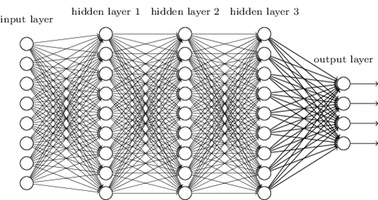
\includegraphics[width=0.9\columnwidth]{nn} 
    \caption{Una rete neurale profonda}
    \label{img:nn}
\end{figure}

\subsection*{Come la rete impara}
La rete impara attraverso l'analisi della sua \textit{loss function}. La \textit{loss function} è una funzione che ci dice quanto la nostra rete è buona per un determinato compito. Per capirlo intuitivamente, essa prende ogni dato in input, lo computa attraverso la rete neurale, lo si sottrae al numero che ci aspettiamo sia il risultato e ne prendiamo il quadrato. Dati quindi $y$ il numero che ci aspettiamo, $\hat{y}$ il numero che otteniamo dalla computazione della rete, $i$ l'indice dell'esempio che stiamo prendendo in considerazione: 
\[L(y, \hat{y})=\frac{1}{m}\sum_{i=1}^{m}(y_i - \hat{y}_i)^2 \]
otteniamo la "distanza" dal risultato che vorremmo ottenere. Imparare diventa quindi un problema di minimo, ovvero vogliamo trovare un risultato che minimizzi la \textit{loss function}. A questo scopo si utilizzano la discesa del gradiente e la \textit{backward propagation}

\subsubsection*{Discesa del gradiente}
Il metodo di discesa del gradiente è una tecnica che consente di determinare i punti di massimo e di minimo di una funzione a più variabili.
\\Pensando ad una funzione $f(x)$ con $x\in \Re^n$, la direzione di massima discesa (ovvero la direzione verso la quale la funzione "scende" più rapidamente) in un punto $\bar{x}$ è dato dall'opposto del suo gradiente in quel punto, ovvero: $p_k:=-\nabla f(\bar{x})$. Questa scelta garantisce che la soluzione tenda ad un punto di minimo di $f$. Il metodo del gradiente prevede dunque di partire da una soluzione iniziale $x_0$ scelta arbitrariamente e di procedere in maniera iterativa aggiornandola come:
\[x_{k+1} = x_k + \alpha_kp_k\]
dove $\alpha_k\in \Re^+$ corrisponde alla lunghezza del passo di discesa, la cui scelta diventa quindi cruciale nel determinare la velocità con cui l'algoritmo converge alla soluzione richiesta.

\subsubsection*{\textit{Backward propagation}}
La propagazione all'indietro viene utilizzata dagli algoritmi di discesa del gradiente per aggiustare i pesi dei neuroni calcolando il gradiente della \textit{loss function}. In pratica, l'algoritmo di ottimizzazione di una rete neurale ripete un ciclo costituito da due fasi: propagazione e aggiornamento dei pesi. Quando un vettore in input viene dato in pasto alla rete, viene propagato "in avanti" attraverso la rete, strato su strato, fino a che raggiunge lo strato di uscita. A questo punto l'output viene paragonato col risultato aspettato usando una \textit{loss function}. A questo punto, l'errore che è risultato viene calcolato per ognuno dei neuroni dello strato di output, dopodiché viene propagato dallo strato di uscita all'indietro nella rete, fino ad associare a tutti i neuroni un valore d'errore che riflette il loro contributo all'output originale. 
\medskip
\\La \textit{backpropagation} quindi usa questi valori per calcolare il gradiente della \textit{loss function}. Nella seconda fase, questo gradiente viene dato in pasto al metodo di ottimizzazione, che lo usa per aggiornare i pesi, per cercare di minimizzare la funzione di perdita.

\medskip
\medskip
\medskip
Per il mio studio mi sono fin da subito concentrato sulle \textit{deep neural network}, ovvero reti neurali che sono composte da molti strati che comunicano fra loro. Nelle prossime sezioni mostrerò alcuni modelli ben definiti e le architetture che poi ho usato nel mio progetto.



\section{Excursus sulle \textit{deep network architectures}}
Quasi tutto il progresso sull'apprendimento profondo degli ultimi anni per la branca del \textit{computer vision} può essere riassunto in poche architetture di reti neurali.
Tralasciando in questa sede tutta la matematica e il codice che vi sta dietro, vorrei introdurre il lettore a comprendere come queste reti funzionano e perché.
\medskip
\\Prendiamo ad esempio la libreria Keras\cite{prod:keras}: questa libreria, capace di lavorare come \textit{wrapper} attorno a \grayname{Tensorflow}\cite{prod:tensorflow}, \grayname{CNTK}\cite{prod:CNTK} e \grayname{Theano}\cite{prod:Theano} offre sei modelli già allenati, \textit{built-in} al suo interno:
\begin{itemize}
	\item \textbf{VGG16}
	\item \textbf{VGG19}
	\item \textbf{MobileNet}
	\item \textbf{ResNet50}
	\item \textbf{Inception v3}
	\item \textbf{Xception}
\end{itemize}

Le reti VGG seguono l'archetipo - ora in parte superato - delle \textit{convolutionary nets}: sono costituite infatti da una serie di strati convoluzionali, di \gls{max-pooling} e con uno strato \textit{fully-connected} per classificazione nel fondo. Le MobileNet sono una versione ottimizzata per le applicazioni mobile della Xception. Le ultime tre, invece, ridefiniscono veramente il modo in cui pensiamo alle reti neurali.
\medskip

\subsection{ResNet}
La domanda chiave che gli sviluppatori si sono fatti pensando al modello di questa rete è stata: \textit{Perché ogni rete profonda ha una prestazione peggiore man mano che si aggiungono strati?}\cite{site:intuitive_guide_DNN_architecture}
Infatti ci si può aspettare che, dati $n$ strati, una rete con $n+1$ abbia la stessa identica accuratezza di quella a $n$. Tuttavia la pratica smentisce questa osservazione, mettendo in risalto l'opposto.
\medskip
\\L'ipotesi che gli autori di ResNet hanno fatto è stata che \textit{mappings} diretti sono difficili da imparare. Così hanno proposto una modifica: al posto di cercare di stimare una funzione $G$ che dato un $x$ restituisca $G(x)$, è meglio apprendere la \textit{differenza} tra i due - anche chiamato residuo, da cui il nome. Di conseguenza, per calcolare $G(x)$ a partire da $x$ basta aggiungere il suo residuo.\\
Quindi, detto:
\[F(x)=G(x)-x\]
il nostro residuo, al posto di apprendere $G(x)$ direttamente, la rete cercherà di imparare
\[F(x)+x\].
Questo ci dà l'opportunità di introdurre il \textit{ResNet block} (figura \ref{img:resnet_block}):
\begin{figure}[!h] 
	\centering 
	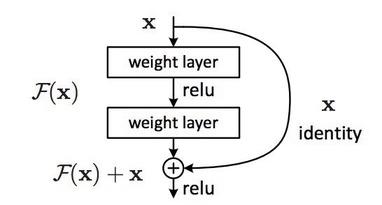
\includegraphics[width=0.9\columnwidth]{resnet_block} 
	\caption{Blocco ResNet}
	\label{img:resnet_block}
\end{figure}
ogni blocco è costituito da una serie di strati e da una "scorciatoia", che aggiunge l'input del blocco stesso al suo output. L'operazione di aggiunta è fatta per ogni elemento, e se input e output sono di dimensioni diverse viene eseguito un \textit{\gls{zero-padding}} oppure una proiezione (via \gls{convoluzioni} 1x1) per portare l'input alla stessa dimensione dell'output. Intuitivamente è molto più semplice imparare mandando $F(x)$ a 0 lasciando l'output a $x$ piuttosto di cercare di imparare una trasformazione identità da zero. In altre parole, ResNet dà uno strato di riferimento - $x$, per l'appunto - da cui iniziare ad imparare.
\medskip
\\Quest'idea funziona molto bene nella pratica. Mentre i modelli precedenti soffrivano del cosiddetto \gls{vanishing gradient}, qui invece si possono sfruttare delle scorciatoie verso gli strati precedenti: reti da 50, 100 o addirittura 1000 strati di profondità hanno ancora delle ottime performance.

\subsection{Inception}
La domanda chiave che invece gli sviluppatori della famiglia delle Inceptions si sono fatti è stata: \textit{come possiamo scalare efficientemente le reti neurali senza aumentare il costo computazionale?}\cite{site:intuitive_guide_DNN_architecture} 
Il paper originale\cite{site:inception} si concentra sulla definizione di un "Inception module", che ha come base due concetti fondamentali: le operazioni sugli strati e la possibile riduzione della dimensione di ognuno. Ma andiamo con ordine:

\subsubsection*{Più operazioni per strato}
In una \textit{conv net} tradizionale ogni livello estrae nuove informazioni dallo strato precedente per trasformare i dati in ingresso in una rappresentazione più fruibile per la rete. Tuttavia, ogni tipologia di livello estrae informazioni diverse: l'output di una convoluzione di dimensione 5x5 è diverso da quello di uno a 3x3, ed è diverso anche da uno dove si opera un \textit{max-pooling}. Come possiamo sapere se una certa trasformazione in un certo strato sta estraendo informazioni utili?
\medskip 
\\L'idea è stata di lasciare la rete decidere quali scegliere: il modulo Inception esegue multiple e diverse trasformazioni sullo stesso input in maniera parallela, concatenando poi i risultati in un output singolo. In pratica, come mostrato in figura \ref{img:inception_module}, per ogni strato Inception esegue una convoluzione 5x5, 3x3 e un \textit{max-pooling}. Lo strato successivo si occupa quindi di decidere se e come usare ogni informazione così tracciata.
\begin{figure}[!h] 
	\centering 
	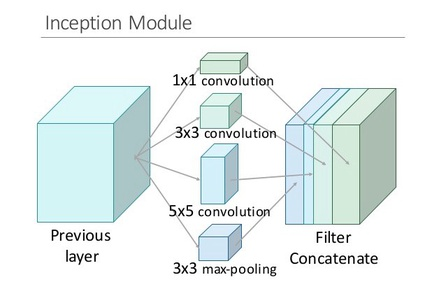
\includegraphics[width=0.9\columnwidth]{inception_module} 
	\caption{Modulo Inception}
	\label{img:inception_module}
\end{figure}

\subsubsection*{Riduzione dimensionale}
Facendo così tuttavia si introduce un problema: si è ingrandita drasticamente la computazione. Per ogni filtro aggiunto bisogna fare la convoluzione di tutti gli strati di input precedenti per calcolare un singolo output. Questo porta ad un aumento quadratico o addirittura maggiore del numero dei filtri per strato. Ci si rende facilmente conto che questo non è sostenibile.
\medskip
\\Ecco quindi la soluzione: gli autori hanno pensato ad una convoluzione 1x1 per "filtrare" la profondità degli output. Se si considera una convoluzione 1x1 su un singolo strato si ha una valutazione di un valore alla volta. Tuttavia, vista su più \gls{canali}, essa può estrarre informazioni "spaziali" e comprimerli ad una dimensione inferiore. Facciamo un esempio: usando 20 filtri 1x1, un input di dimensione 64x64x100 può essere compresso a 64x64x20. Così facendo gli autori del modello sono stati capaci di allocare più trasformazioni per strato in parallelo, avendo una rete simultaneamente ampia (per via del parallelismo) e profonda (grazie al grande numero di strati).
\begin{figure}[H] 
	\centering
	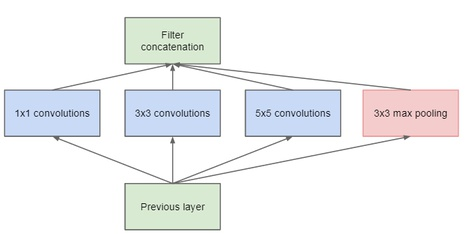
\includegraphics[width=0.6\columnwidth]{inception_module_naive} 
	\caption{Concezione iniziale del modulo Inception}
	\label{img:inception_module_naive}
\end{figure}
\begin{figure}[H] 
	\centering
	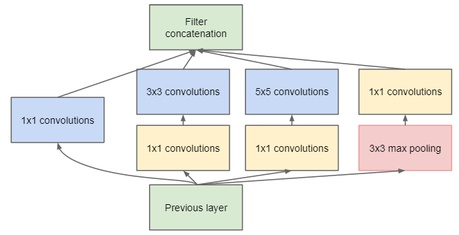
\includegraphics[width=0.6\columnwidth]{inception_module_reduced} 
	\caption{Modulo Inception con riduzione}
	\label{img:inception_module_reduced}
\end{figure}
Inception ha dimostrato la potenza delle architetture composte da "reti dentro a reti", aggiungendo un altro gradino importante alla potenza rappresentale delle reti neurali.
\begin{figure}[H] 
	\centering
	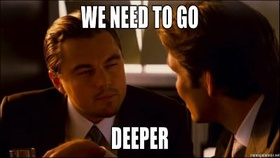
\includegraphics[width=0.6\columnwidth]{need_go_deeper} 
	\caption{Meme letteralmente citato dall'articolo originale su Inception}
	\label{img:need_go_deeper}
\end{figure}

\subsection*{Xception}
Xception sta per \textit{extreme inception} e porta il concetto del modulo Inception ad un estremo. L'ipotesi da cui si sviluppa questa rete è: \textit{la correlazione tra i canali e quella spaziale sullo stesso frame è sufficientemente bassa da poter preferire di non mapparli assieme}.
Cosa vuol dire? Nelle tradizionali reti a convoluzione, gli strati cercano correlazioni sia in profondità che in larghezza (ovvero sullo stesso frame). Con Inception si ha avuta una prima separazione: usando una convoluzione 1x1 si può mappare l'input originale in vari input separati, sui quali poi poter eseguire diversi tipi di trasformazione. Xception porta il concetto un po' oltre: al posto di partizionare l'input in tanti piccoli pezzi, questa partiziona ogni canale separatamente, quindi esegue una convoluzione 1x1 in profondità per catturare correlazioni tra i canali.
\begin{figure}[H] 
	\centering
	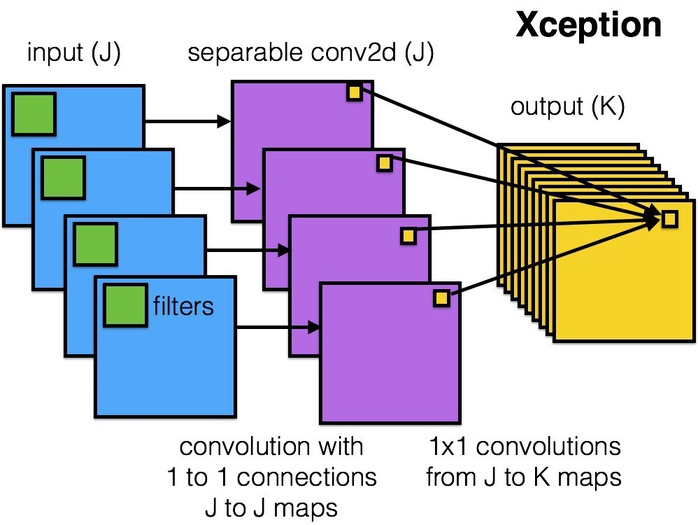
\includegraphics[width=0.6\columnwidth]{xception} 
	\caption{Modulo Xception}
	\label{img:xception_module}
\end{figure}
Possiamo immaginare questa operazione considerando la ricerca di correlazione tra spazi bidimensionali e poi su unidimensionali. Il che è intuitivamente più semplice che cercarle in uno spazio direttamente tridimensionale.
\medskip
\\Questo modello è molto recente - è uscito nell'aprile del 2017 - e già ha risultati promettenti, soprattutto per quanto riguarda l'efficienza computazionale con un più alto numero di \gls{classi} da analizzare.


\section{Il \textit{deep learning} applicato all'\textit{object detection}}
Con l'aumento delle auto a guida autonoma, dei sistemi di videosorveglianza \textit{smart}, del riconoscimento facciale e di molti altri campi di utilizzo, la richiesta di sistemi di  \textit{detection} è andata via via sempre aumentando. Tuttavia, questi sistemi non solo richiedono di classificare ogni oggetto in un'immagine, ma anche di trovarlo, disegnandogli un rettangolo attorno. Come si può immaginare, questo compito è nettamente più complesso della semplice \textit{image classification}. Fortunatamente i migliori approcci usati oggi giorno provengono principalmente da estensioni dei modelli già esistenti e derivati dalla classificazione.
%\vspace{1.5\baselineskip}
\medskip
\\Circa un anno fa Google ha rilasciato una nuova \glslink{api}{API} di \textit{object detection} e, assieme ad essa, ha fornito anche una serie di architetture - con i relativi pesi già allenati - per alcuni specifici modelli:
\begin{itemize}
	\item Single Shot Multibox Detector (SSD) con le MobileNets
	\item SSD con Inception V2
	\item Region-Based Fully Convolutional Networks (R-FCN) con Resnet 101
	\item Faster R-\glslink{cnn}{CNN} con Resnet 101
	\item Faster \glslink{rcnn}{R-CNN} con Inception Resnet v2
\end{itemize}
Dopo aver intrapreso uno studio preliminare riguardo le varie architetture, ho preferito concentrarmi su due in particolare: la Faster R-CNN con Inception Resnet V2 e la SSD con Inception V2. Queste infatti sono disponibili all'interno dell'API di \textit{object detection}\cite{prod:tensorflow_o_d_api} di \grayname{Tensorflow}\cite{prod:tensorflow} e hanno reso il mio approccio alla materia molto meno drastico.

\subsection{Cosa sono il \textit{transfer learning} e il \textit{fine tuning}}
Per usufruire di queste reti ho dovuto utilizzare il \textit{transfer learning}. Molte poche persone allenano un'intera \textit{conv net} da zero con inizializzazione casuale, poiché è raro avere a disposizione un \textit{dataset} così ampio. Piuttosto, si tende ad utilizzare una rete già allenata. quindi usare i pesi - ovvero le informazioni che già ha imparato da un particolare insieme di dati - di questa come di partenza per la propria. 
\medskip
\\In particolare, per questo progetto ho utilizzato il \textit{fine tuning}: \grayname{Tensorflow} mette a disposizione i pesi "congelati" di tutti gli strati eccetto del penultimo. Così facendo, possiamo allenare la nostra rete ad imparare la rappresentazione del solo ultimo strato, utilizzando il \textit{dataset} personale. Questo è ovviamente possibile solamente se c'è una certa continuità dell'obiettivo della rete: sfruttare il \textit{fine tuning} per imparare una voce utilizzando come base di partenza il grafo di una \textit{object detection} è inutile e controproducente.

\subsection{Faster R-CNN}
La Faster R-CNN è l'architettura di riferimento nell'apprendimento profondo, in particolare per quanto riguarda l'\textit{object detection} ed è di riferimento per altre architetture, in particolare anche per la SSD. Tuttavia, non la si può realmente capire se prima non si dà una rapida occhiata alle sue predecessore, la R-CNN e la Fast R-CNN.

\subsubsection*{R-CNN}
La R-CNN, ovvero la \textit{Region-based Convolutional Neural Network} consiste di tre passaggi:
\begin{enumerate}
	\item scansiona l'immagine di input e cerca oggetti possibili con un algoritmo di ricerca selettiva, generando circa 2000 \textit{region proposal}, regioni da "proporre" agli strati successivi;
	\item esegue una rete convoluzionale su ognuna di esse;
	\item prende l'output di ogni CNN e lo dà in pasto a:
	\begin{itemize}
		\item una \glslink{svm}{SVM} per classificare le regioni;
		\item una \gls{regressione lineare} per creare un riquadro attorno all'oggetto, se esiste.
	\end{itemize}
\end{enumerate}
Gli step sono mostrati nella figura \ref{img:r-cnn_architecture}.
\begin{figure}[H] 
	\centering
	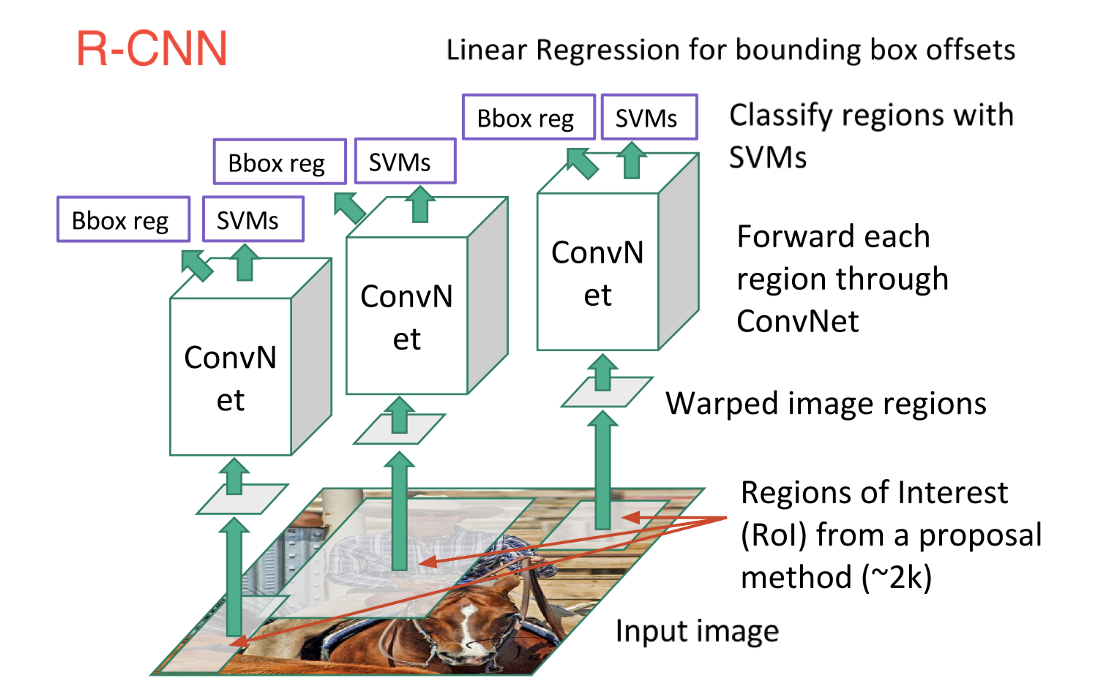
\includegraphics[width=0.9\columnwidth]{r-cnn} 
	\caption{Architettura R-CNN}
	\label{img:r-cnn_architecture}
\end{figure}
Intuitivamente, prima di tutto si trovano le possibili regioni in cui può essere contenuto un oggetto, poi si estraggono le informazioni ad esse associate, poi in base a queste si classificano. Si è trasformato un problema di \textit{object detection} in uno di classificazione: era un approccio molto intuitivo ma allo stesso tempo lento e oneroso.

\subsubsection*{Fast R-CNN}
Questa architettura è stata la diretta discendente della R-CNN, ma ha aumentato la sua velocità con due fattori chiave:
\begin{itemize}
	\item esegue l'estrazione di informazioni una volta prima di creare le regioni da proporre; così facendo può permettersi di eseguire una sola CNN al posto di doverne eseguire una per ogni regione;
	\item sostituisce la SVM con un \textit{layer} \gls{softmax}.
\end{itemize}
La nuova architettura si mostrava quindi come in figura \ref{img:fast-r-cnn_architecture}.
\begin{figure}[!ht] 
	\centering
	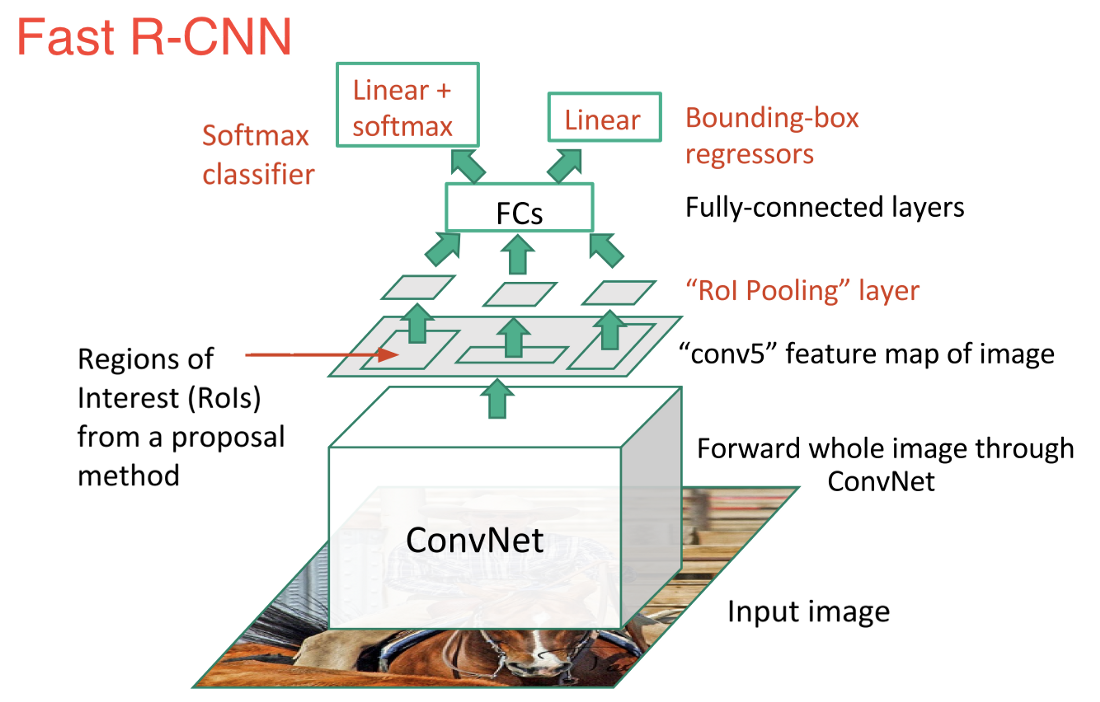
\includegraphics[width=0.9\columnwidth]{fast-r-cnn} 
	\caption{Architettura Fast R-CNN}
	\label{img:fast-r-cnn_architecture}
\end{figure}
Come si può vedere in figura, le \textit{region proposals} sono generate a partire dall'ultimo strato di informazioni ricavate dalla rete e non dall'immagine in sé. \'E quindi possibile allenare una singola CNN per l'immagine intera. Inoltre, al posto di usare molte SVM per classificare ogni classe, c'è un solo \textit{layer} \textit{softmax} che genera una probabilità diretta.
\medskip
\\La Fast R-CNN era molto più veloce della precedente, ma l'algoritmo di \textit{selective search} era ancora troppo lento.

\subsubsection*{Faster R-CNN}
Per risolvere questo ultimo collo di bottiglia si è adottato, al posto dell'algoritmo di ricerca selettiva, una rete neurale veloce. In particolare, una RPN, \textit{Region Proposal Network}:
\begin{itemize}
	\item viene generata una \textit{sliding window} di dimensione 3x3 posizionata sull'ultimo strato della CNN iniziale, che si muove lungo la mappa e ne restituisce una versione più piccola, ridotta (ad esempio a 256-d);
	\item per ogni \textit{sliding window} genera più possibili regioni basate su alcune \textit{boxes} di proporzione prestabilita;
	\item ogni regione proposta consiste di:
	\begin{itemize}
		\item un punteggio, \textit{score}, col quale viene valutata la \textit{box} trovata;
		\item le effettive quattro coordinate della scatola;
	\end{itemize}
\end{itemize}
In altre parole, si guarda in ogni posto proposto dall'ultimo strato della \textit{conv net}, si considerano $k$ diverse scatole centrate su ognuna di esse: una alta, una larga, una grande, una piccola, ecc. Per ognuna di queste viene generato un punteggio, una sorta di \textit{likelihood}. 
Da notare, infine, che anche se la RPN ha come output delle \textit{bounding boxes}, essa non aspira a classificare un potenziale oggetto: semplicemente propone delle regioni in cui ci potrebbe essere. Se una scatola ha un punteggio sufficiente, viene quindi passata avanti come \textit{region proposal}.
\begin{figure}[!ht] 
	\centering
	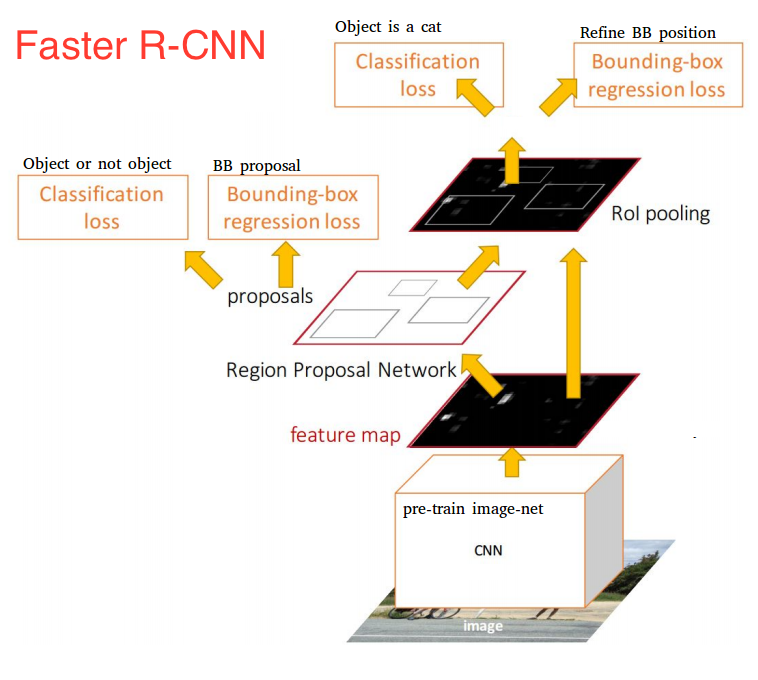
\includegraphics[width=0.7\columnwidth]{faster-r-cnn} 
	\caption{Architettura Faster R-CNN}
	\label{img:faster-r-cnn_architecture}
\end{figure}

\subsection{SSD}
Mentre la Faster R-CNN prima generava delle regioni, per poi usare un \textit{fully connected layer} per classificarle, la SSD fa tutto questo in un solo colpo. Da qui il nome, Single-Shot Detector.
In pratica, data un'immagine appartenente ad un \textit{set} con delle \textit{ground truth label}, ovvero delle immagini etichettate, la SSD fa questi passaggi:
\begin{enumerate}
	\item prima passa l'immagine attraverso una serie di strati convoluzionali, raggruppando più insiemi di mappe con informazioni a diverse misure (ad esempio 10x10, poi 6x6, e così via);
	\item per ogni \textit{location}, per ognuna delle \textit{feature maps}, usa un filtro con una convoluzione 3x3 per valutare insiemi più piccoli di scatole; questo è più o meno quello che viene fatto con le scatole della Faster R-CNN;
	\item per ogni scatola, valuta contemporaneamente:
	\begin{itemize}
		\item un offset per una possibile \textit{bounding box};
		\item la probabilità collegata ad una classe;
	\end{itemize}
	\item durante l'allenamento, fa il match delle scatole trovate con quelle effettivamente etichettate, basato su \glslink{iou}{IoU}.
\end{enumerate}

L'allenamento di una SSD può tuttavia essere un'impresa. Se nella Faster avevamo infatti una minima scelta basata sulla probabilità, qui le regioni proposte sono \textit{tutte} quelle possibili all'interno dell'immagine. Di conseguenza quasi sicuramente molte delle scatole trovate sono da scartare. Per migliorare questo aspetto sono stati introdotti due approcci:
\begin{itemize}
	\item usare una \gls{non-maximum suppression} per raggruppare assieme alcune scatole che sono molto sovrapposte;
	\item usare l'\gls{hard negative mining} per bilanciare le classi durante l'allenamento.
\end{itemize}

\subsection{Considerazioni finali}
La SSD è una rete molto veloce e ha una performance paragonabile alle altre. Tuttavia, nonostante sia una tra le più complesse architetture e una tra le più lente, allo stato attuale la Faster è tra le migliori in termini di accuratezza\footfullcite{site:COCO-trained-model-statistics}. Per questo motivo, dopo uno studio preliminare dell'argomento, visto il \textit{dataset} a disposizione e vista la mancanza di tempo per poter personalmente testare il modello migliore, ho deciso di utilizzare questa architettura. In seguito discuterò di come ho personalizzato questa rete, in base ai risultati sul mio particolare problema.